本アプリの依頼側、配達側、店舗側そして管理側の各機能設計について記述する。
\subsection{機能概要図}
以下に示す図は本アプリの機能概要である。

\subsubsection{ログイン関連機能}
図\ref{fig:ログイン関連機能}は、ログイン関連機能の概要図である。
\begin{figure}[H]
  \centering
  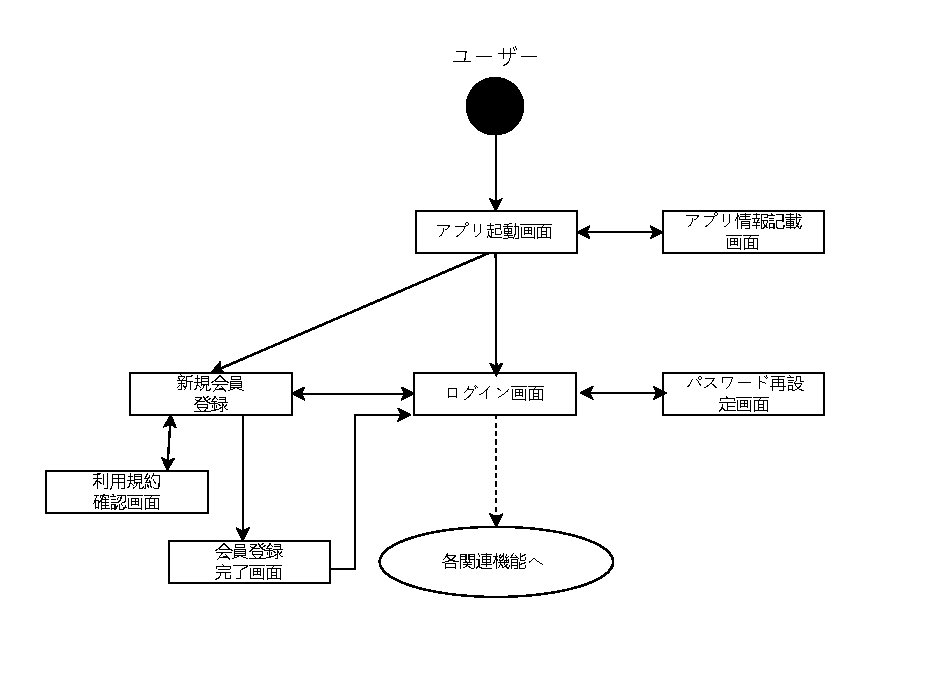
\includegraphics[width=0.75\textwidth]{./ログイン関連機能.pdf}
  \caption{ログイン関連機能}
  \label{fig:ログイン関連機能}
\end{figure}



\subsection{共通機能}
本アプリの依頼側、配達側、店舗側そして管理側の共通の機能設計を以下に記述する。
\subsubsection{新規会員登録機能}
依頼側と配達側、店舗側が利用規約に同意し、情報を入力し、その情報に不備がなく、送信されたメールで本人確認を行うこ
とで、新規会員登録ができる機能である。また、入力情報として、配達側と依頼側は名前、性別、歳、住所、メールアドレス
、電話番号、パスワード、パスワード(確認)を、店舗側は店舗所在地、飲食店営業許可書のファイルおよび写真、メールア
ドレスまたは電話番号、パスワード、パスワード(確認)を入力する。

\begin{figure}[H]
  \centering
  \includegraphics[width=0.75\textwidth]{./新規会員登録機能.pdf}
  \caption{新規会員登録機能}
  \label{fig:新規会員登録機能}
\end{figure}



\subsection{依頼側}



\subsection{配達側}

\subsection{店舗側}

\subsection{管理側}

